\documentclass{article}
\usepackage[preprint]{neurips_2025}
\usepackage[utf8]{inputenc}
\usepackage[T1]{fontenc}
\usepackage{graphicx}
\usepackage{booktabs}
\usepackage{amsmath,amssymb}
\usepackage{hyperref}
\usepackage{xcolor}
\hypersetup{hidelinks}

\title{Cross-Model Embedding Adapters, Measured on Retrieval}

\makeatletter\renewcommand{\@noticestring}{}\makeatother
\author{Han Xiao \\
Jina AI \textit{by} Elastic \\
\texttt{han.xiao@jina.ai}}

\begin{document}
\maketitle

\begin{abstract}
A closed-form map between two text embedding spaces costs one SVD and is meant to restore retrieval across a model switch without re-embedding a corpus. We measure what it restores over 56 directed pairs from eight embedding models of six families, evaluated on 13 NanoBEIR tasks across five random validation-test splits. An orthogonal rotation fitted on 5{,}000 paired texts recovers 0.766 of the source model's nDCG@10 on average and beats keeping the old index on 1 of 56 pairs, where the two models are consecutive checkpoints of one lineage. Adding the centring and global scale of Plato's Key raises the mean from 0.4998 to 0.5462 when selected on validation, winning 18 of 56 pairs significantly with zero significant losses and matching two-sided Ridge CCA without touching the corpus. When fixed without validation, Plato's Key drops 0.0807 nDCG@10 on anisotropic targets because adding the target mean injects query-independent hubness bias; subtracting only the source mean removes this failure, reaching 0.5336 with zero hyperparameters and outperforming both rotation and fixed affine maps at every calibration budget from 50 to 5{,}000 texts. Two pre-fit diagnostics predict deployment behaviour: frame correlation $\rho$ correlates 0.951 with the identity baseline and $-0.862$ with map gain, while source anisotropy $\kappa_s$ correlates 0.882 with affine gain over rotation and accounts for most directional asymmetry, whose variance share falls from 0.441 under rotation to 0.053 under affine alignment. Chaining two maps through a third model retains a median 0.977 of direct retrieval over 336 triples, a single source-centred generalized-Procrustes hub across all eight models reaches 0.5345 against 0.5336 for pairwise fitting, and one-sided low-rank compression to 256 components keeps 0.819 of full-rank affine retrieval. Finally, mixing newly re-indexed documents with corpus-adapted legacy vectors in one raw-cosine index collapses retrieval by up to 0.247 nDCG@10 at 25\% migration due to background cosine shift; per-query z-scoring of the top-100 hits per shard eliminates this drop.
\end{abstract}

\section{Introduction}

Switching embedding models invalidates an existing vector index. Queries encoded by a new model no longer match documents stored by the old one, and re-embedding millions of passages costs days of GPU compute. A closed-form linear map fitted on a few thousand unlabeled paired texts bridges the two spaces in under half a second on CPU without touching model weights. Orthogonal Procrustes alignment dates to cross-lingual word translation \citep{conneau2018word,artetxe2018vecmap} and has recently been evaluated on dense retrieval \citep{vejendla2025drift,zhao2026bill,xiao2026adapters}.

Two recent lines of work sharpen what remains unmeasured. First, \citet{zhao2026bill} point out that approaching the target model's score is the wrong bar for an operator deciding whether to migrate; the honest comparison is whether the adapted query beats keeping the old index. Second, Plato's Key \citep{platoskey2026} shows that an affine map comprising centring, an orthogonal rotation, and one global Frobenius scale transfers factual recall across frozen LLM hidden states, chains across three models, compresses to 256 principal components, and recovers dark memories that the recipient model fails to recall on its own.

We evaluate the Plato's Key estimator and protocol directly on text retrieval across eight embedding models from six vendors, spanning 768 to 2048 dimensions and 56 directed pairs. Our measurements uncover four mechanisms specific to retrieval that separate it from hidden-state transfer. First, adding the target mean helps when an anisotropic source maps into an isotropic target, but hurts by 0.0807 nDCG@10 when the target is itself anisotropic, because cosine scoring against an uncentred corpus turns the target mean into a query-independent hubness bias. Omitting the target shift while keeping source centring yields a zero-hyperparameter map that dominates both uncentred rotation and fixed Plato's Key across all calibration sizes. Second, directional asymmetry is driven by source and target anisotropy rather than by dimension mismatch; correcting anisotropy reduces antisymmetric variance from 44.1\% to 5.3\%. Third, when fitted on all 5{,}000 calibration texts to convergence, a single shared Platonic hub across all eight models matches or exceeds 56 pairwise maps. Fourth, progressive zero-downtime migration into a mixed index fails catastrophically under raw cosine scoring because adapted vectors have an attenuated cosine peak and shifted background mean, and a five-line per-shard top-100 z-score normalizer restores a monotone migration curve.

\section{Methods}

Let $\mathbf{X}\in\mathbb{R}^{n\times d_s}$ and $\mathbf{Y}\in\mathbb{R}^{n\times d_t}$ denote L2-normalized embeddings of the same $n$ calibration texts produced by a source model and a target model. A query $\mathbf{q}\in\mathbb{R}^{d_s}$ is mapped into $\mathbb{R}^{d_t}$, renormalized, and scored by cosine similarity against native target documents $\mathbf{d}\in\mathbb{R}^{d_t}$. All one-sided maps leave the stored document index untouched.

\begin{figure}[t]
\centering
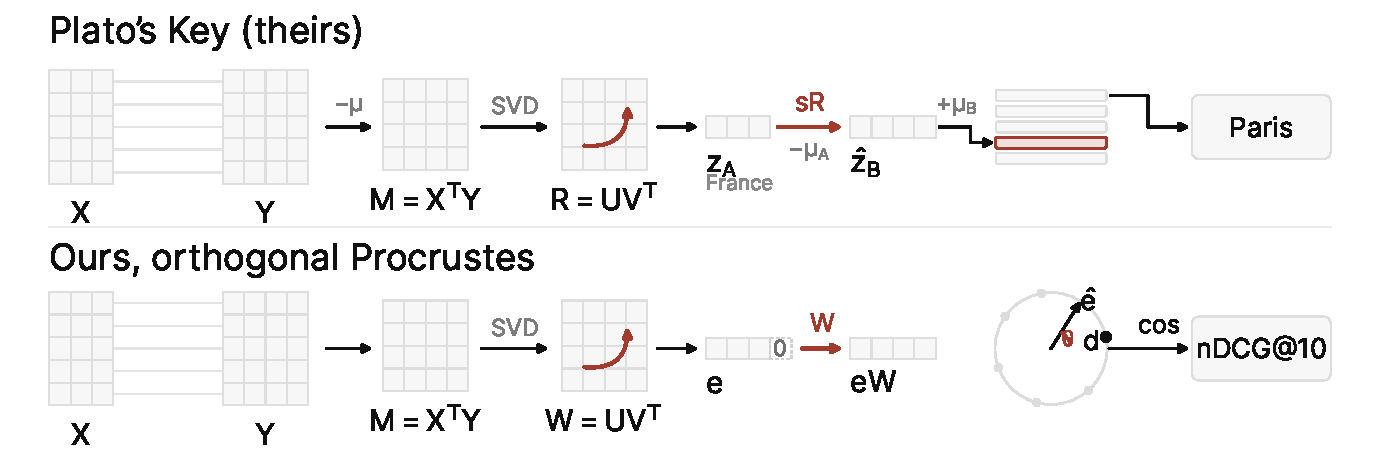
\includegraphics[width=\textwidth]{method.pdf}
\caption{Two closed-form maps over one SVD skeleton. Top, Plato's Key \citep{platoskey2026}: an affine map between frozen LLM hidden states that centres, rotates, rescales, and re-centres before substituting the key into a later transformer layer. Bottom, orthogonal Procrustes \citep{xiao2026adapters}: a pure semi-orthogonal map between pooled text embeddings scored by cosine similarity against a frozen index.}
\label{fig:methods}
\end{figure}

\subsection{Closed-form and learned adapters}

\paragraph{Orthogonal Procrustes.} Minimizes $\lVert\mathbf{X}\mathbf{R}-\mathbf{Y}\rVert_F$ over semi-orthogonal matrices via one thin SVD of the cross-covariance $\mathbf{X}^\top\mathbf{Y}=\mathbf{U}\boldsymbol{\Sigma}\mathbf{V}^\top$, giving $\mathbf{R}=\mathbf{U}\mathbf{V}^\top\in\mathbb{R}^{d_s\times d_t}$. When $d_s\neq d_t$, thin SVD directly yields orthonormal rows when $d_s<d_t$ and orthonormal columns when $d_s>d_t$, matching zero-padding without extra memory.

\paragraph{Affine Procrustes (Plato's Key).} Centres both sides on the calibration means $\boldsymbol{\mu}_X,\boldsymbol{\mu}_Y$, fits the orthogonal rotation $\mathbf{R}_c$ on $\tilde{\mathbf{X}}=\mathbf{X}-\boldsymbol{\mu}_X$ and $\tilde{\mathbf{Y}}=\mathbf{Y}-\boldsymbol{\mu}_Y$, rescales by the Frobenius spread ratio $s=\lVert\tilde{\mathbf{Y}}\rVert_F/\lVert\tilde{\mathbf{X}}\rVert_F$, and restores $\boldsymbol{\mu}_Y$:
\begin{equation}
\hat{\mathbf{z}} = \mathrm{norm}\!\left(\boldsymbol{\mu}_Y + s\,(\mathbf{z}-\boldsymbol{\mu}_X)\mathbf{R}_c\right).
\label{eq:affine}
\end{equation}
We evaluate both the fixed estimator (\texttt{affine-cs}), a least-squares scalar variant $s_{\mathrm{LS}}=\mathrm{tr}(\tilde{\mathbf{X}}^\top\tilde{\mathbf{Y}}\mathbf{R}_c^\top)/\lVert\tilde{\mathbf{X}}\rVert_F^2$ (\texttt{affine-ls}), and the four-way validation-selected family over centring on or off and scale on or off (\texttt{affine}).

\paragraph{Source-centred Procrustes.} Fits the same centred rotation $\mathbf{R}_c$ as Equation~\eqref{eq:affine} and subtracts $\boldsymbol{\mu}_X$ at inference, but sets $\boldsymbol{\mu}_Y=\mathbf{0}$ and $s=1$:
\begin{equation}
\hat{\mathbf{z}} = \mathrm{norm}\!\left((\mathbf{z}-\boldsymbol{\mu}_X)\mathbf{R}_c\right).
\label{eq:src_centred}
\end{equation}
Subtracting $\boldsymbol{\mu}_X$ prevents an anisotropic source mean from dominating the SVD or collapsing angular spread, while omitting $\boldsymbol{\mu}_Y$ prevents the target mean from biasing cosine retrieval toward hub documents. Equation~\eqref{eq:src_centred} requires zero hyperparameters and no validation queries.

\paragraph{Alternative linear, kernel, and neural baselines.} We compare against closed-form centred ridge regression $\mathbf{A}=(\frac{1}{n}\tilde{\mathbf{X}}^\top\tilde{\mathbf{X}}+\lambda\mathbf{I})^{-1}\frac{1}{n}\tilde{\mathbf{X}}^\top\tilde{\mathbf{Y}}$ with $\lambda\in\{10^{-5},\dots,10^{-1}\}$ and optional Frobenius rescaling, regularized ZCA-whitened Procrustes with $\lambda\in\{10^{-2},10^{-1},1\}$, two-sided Ridge CCA at rank $k\in\{32,\dots,512\}$ (which requires re-projecting the document index), RBF kernel ridge regression on 2{,}500 pairs, and two GPU-trained contrastive controls: a linear map and a 3-layer residual MLP with LayerNorm, GELU, and a skip connection initialized at the closed-form affine solution, both trained with InfoNCE plus cosine loss and early stopping on a 10\% calibration holdout. Random Haar semi-orthogonal maps, Procrustes fitted on shuffled pairs, and the identity map serve as controls.

\subsection{Pre-fit diagnostics}

Two scalar statistics computed on calibration pairs before fitting predict adapter behaviour. Frame correlation $\rho=\frac{1}{n}\sum_{i=1}^n\langle\mathrm{pad}(\mathbf{x}_i),\mathrm{pad}(\mathbf{y}_i)\rangle$ measures direct coordinate alignment after padding to $\max(d_s,d_t)$; unlike linear CKA, $\rho$ is sensitive to rotation. Model anisotropy $\kappa(\mathbf{X})=\lVert\boldsymbol{\mu}_X\rVert_2 / \mathrm{RMS}(\mathbf{X}-\boldsymbol{\mu}_X)$ measures how strongly embeddings concentrate in a narrow cone around their mean direction.

\section{Experimental setup}

\begin{table}[t]
\centering
\caption{Eight embedding models from six families evaluated on 13 NanoBEIR tasks. Anisotropy $\kappa$ is measured on the 5{,}000 calibration texts; native nDCG@10 is reported over all 649 queries and the 429 held-out test queries.}
\label{tab:native}
\begin{tabular}{lllrrrr}
\toprule
model & family & backbone & dim & $\kappa$ & all 649 & test 429 \\
\midrule
jina-embeddings-v5-small & jina & qwen3 & 1024 & 0.34 & 0.6706 & 0.6822 \\
jina-embeddings-v5-nano & jina & eurobert & 768 & 0.35 & 0.6669 & 0.6800 \\
Qwen3-Embedding-0.6B & qwen & qwen3 & 1024 & 0.50 & 0.6479 & 0.6558 \\
snowflake-arctic-embed-m-v1.5 & snowflake & bert & 768 & 0.49 & 0.6479 & 0.6529 \\
jina-embeddings-v4 & jina & qwen25vl & 2048 & 0.99 & 0.6466 & 0.6527 \\
jina-embeddings-v3 & jina & xlmr & 1024 & 0.27 & 0.6342 & 0.6401 \\
bge-m3 & bge & xlmr & 1024 & 0.74 & 0.6040 & 0.6156 \\
multilingual-e5-large-instruct & e5 & xlmr & 1024 & 1.82 & 0.6104 & 0.6147 \\
\bottomrule
\end{tabular}
\end{table}

We evaluate eight models spanning six vendors and five pretrained backbones, listed in Table~\ref{tab:native}: four Jina models (v3, v4, v5-nano, v5-small), Qwen3-Embedding-0.6B, bge-m3, multilingual-e5-large-instruct, and snowflake-arctic-embed-m-v1.5. Dimensions span 768, 1024, and 2048, producing 56 directed pairs (17 expanding $d_s<d_t$, 22 equal-width $d_s=d_t$, and 17 compressing $d_s>d_t$) and 336 ordered triples. Each model uses its recommended query prompt and document prompt.

Retrieval is evaluated on all 13 tasks of NanoBEIR-en (649 queries and 56{,}723 documents). Queries are split once per task into one third validation (220 queries) and two thirds test (429 queries) for the primary protocol, and repeated across five random seeds to measure split variance. Calibration uses 5{,}000 unique AG News texts verified to have zero overlap with NanoBEIR, half encoded in query mode and half in passage mode. Following Plato's Key, every method with a free parameter selects it on validation nDCG@10 and reports held-out test nDCG@10. Per-pair significance against orthogonal Procrustes uses a two-sided Wilcoxon signed-rank test over the 13 task means at $\alpha=0.05$.

\section{Results}

\subsection{Adapter comparison across 56 pairs}
\label{sec:main}

\begin{table}[t]
\centering
\caption{Adapter families averaged over 56 directed pairs on the 429 held-out queries. Wins and losses count pairs with a statistically significant difference ($p<0.05$, Wilcoxon over 13 tasks) against orthogonal Procrustes.}
\label{tab:families}
\begin{tabular}{lrrrrr}
\toprule
method & nDCG@10 & /source & /target & wins & losses \\
\midrule
procrustes & 0.5244 & 0.805 & 0.810 & 0 & 0 \\
affine & 0.5718 & 0.882 & 0.882 & 14 & 0 \\
ridgecca & 0.5708 & 0.881 & 0.881 & 12 & 7 \\
SGD-linear & 0.5360 & 0.827 & 0.827 & 7 & 26 \\
SGD-mlp & 0.5232 & 0.807 & 0.807 & 7 & 28 \\
krr-rbf & 0.4764 & 0.735 & 0.732 & 7 & 26 \\
random & 0.0027 & 0.004 & 0.004 & 0 & 42 \\
shuffled & 0.0035 & 0.005 & 0.005 & 0 & 42 \\
identity & 0.0746 & 0.119 & 0.119 & 1 & 39 \\
\bottomrule
\end{tabular}
\end{table}

\begin{figure}[t]
\centering
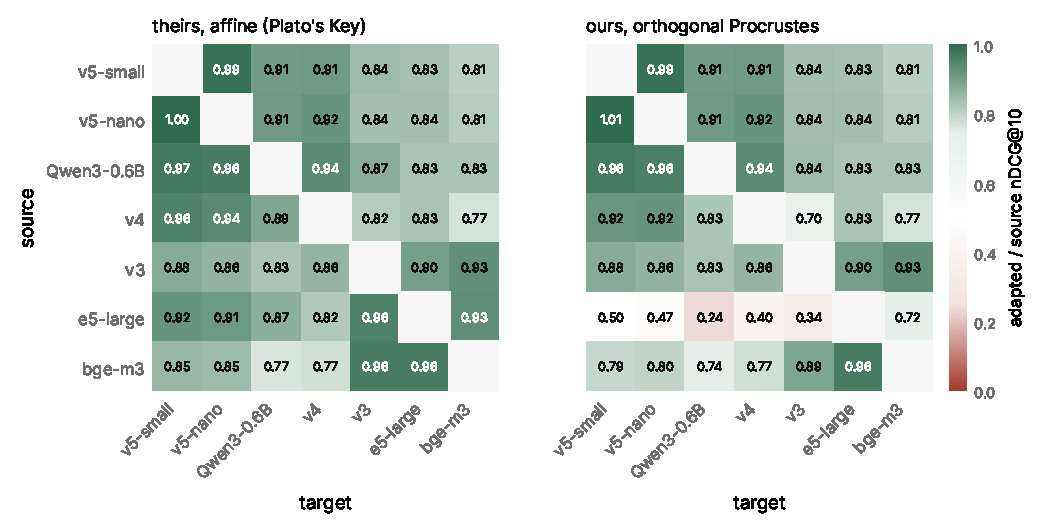
\includegraphics[width=\textwidth]{figs/heatmap.pdf}
\caption{Adapted nDCG@10 as a fraction of the source model's native score over all 56 directed pairs on a shared linear scale from 0 to 1. Left: Plato's Key affine map (validation-selected). Right: orthogonal Procrustes. The two maps agree across low-anisotropy sources, while orthogonal Procrustes collapses across the entire e5-large row (0.14 to 0.72) and the affine map restores it to 0.73 to 0.96.}
\label{fig:heatmap}
\end{figure}

Table~\ref{tab:families} summarizes all 14 methods across the 56 pairs, and Figure~\ref{fig:heatmap} maps retention per pair. Orthogonal Procrustes averages 0.4998 nDCG@10, or 0.766 of the source index, and beats the source index on 1 of 56 pairs, v5-nano to v5-small (0.6838 vs 0.6800). Validation-selected affine alignment (Plato's Key) raises the mean to 0.5462 (0.841 of source), achieving 18 significant wins and zero significant losses against orthogonal Procrustes, and matching two-sided Ridge CCA (0.5440) without modifying the corpus index. Both gradient-trained controls sit below validation-selected affine alignment: SGD linear reaches 0.5345 and the 3-layer residual MLP initialized from the affine solution reaches 0.5301, confirming that contrastive fine-tuning on 5{,}000 pairs does not beat closed-form SVD. Tuned ridge regression (0.5029), whitened Procrustes (0.5210), and RBF kernel ridge (0.4549) also trail. All five random validation-test splits reproduce the same ordering with standard deviation 0.008: validation-selected affine averages $0.5407\pm0.0085$, Ridge CCA $0.5408\pm0.0078$, source-centred Procrustes $0.5304\pm0.0080$, fixed affine $0.5105\pm0.0078$, ridge regression $0.4971\pm0.0082$, and orthogonal Procrustes $0.4931\pm0.0085$.

\subsection{Why Plato's Key needs source centring without target shift on retrieval}
\label{sec:affine}

\begin{figure}[t]
\centering
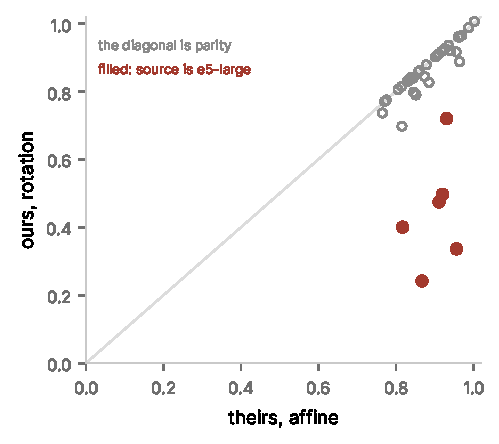
\includegraphics[width=0.44\linewidth]{figs/pair_scatter.pdf}
\hfill
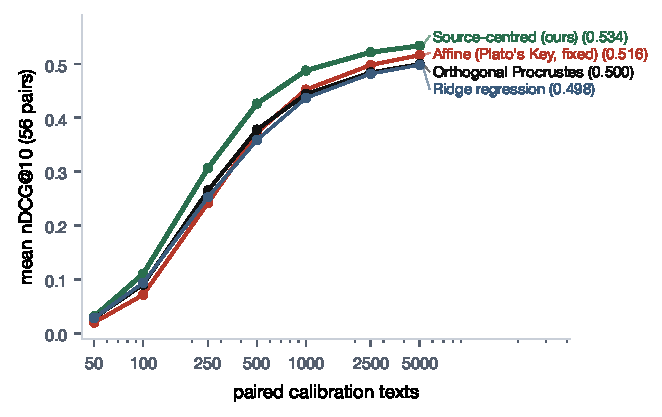
\includegraphics[width=0.53\linewidth]{figs/calsize.pdf}
\caption{Left: validation-selected affine retention against orthogonal Procrustes per directed pair; gains concentrate on high-anisotropy sources (e5-large in red, v4 in slate). Right: mean nDCG@10 across 56 pairs versus calibration budget $n$. Source-centred Procrustes outperforms both rotation and fixed Plato's Key affine at every budget.}
\label{fig:scatter_cal}
\end{figure}

Comparing fixed \texttt{affine-cs} (0.5162) against validation-selected \texttt{affine} (0.5462) exposes a failure mode specific to retrieval. On the 7 pairs whose source is highly anisotropic ($\kappa_s>1$, e5-large), uncentred Procrustes averages 0.2587 because the mean-mean outer product dominates $\mathbf{X}^\top\mathbf{Y}$; centring raises the mean by $+0.2921$ to 0.5508. On the 14 pairs whose target is highly anisotropic ($\kappa_t\ge 0.9$, v4 and e5-large), however, fixed \texttt{affine-cs} drops to 0.4534 against 0.5341 for uncentred Procrustes, a loss of $-0.0807$ (for example v3 to v4 drops from 0.5490 to 0.4703, and bge-m3 to e5-large drops from 0.5917 to 0.4714). The least-squares scale variant \texttt{affine-ls} shrinks the centred signal even further and falls to 0.4752 overall.

The mechanism follows directly from cosine scoring. In Plato's Key, the recipient's next transformer layer expects an activation whose mean and norm match layer $\ell_B$, so adding $+\boldsymbol{\mu}_Y$ and rescaling by $s<1$ is required. In retrieval, adding a large $+\boldsymbol{\mu}_Y$ to a query shifts every query toward the target mean direction and injects a query-independent hubness term $\langle\boldsymbol{\mu}_Y,\mathbf{d}\rangle$ into every document score. Removing the target shift yields source-centred Procrustes (Equation~\eqref{eq:src_centred}), which scores 0.5458 on the 14 anisotropic-target pairs ($+0.0924$ over fixed \texttt{affine-cs} and $+0.0117$ over uncentred Procrustes) and 0.5336 across all 56 pairs with zero hyperparameters. As shown in Figure~\ref{fig:scatter_cal} (right) and Table~\ref{tab:calsize}, source-centred Procrustes dominates uncentred Procrustes, fixed affine, and ridge regression at every calibration budget from $n=50$ to $n=5{,}000$, leading fixed affine by $+0.0536$ at $n=500$ (0.4263 vs 0.3727).

\subsection{Pre-fit diagnostics, dimensional direction, and asymmetry}
\label{sec:diagnostics}

\begin{figure}[t]
\centering
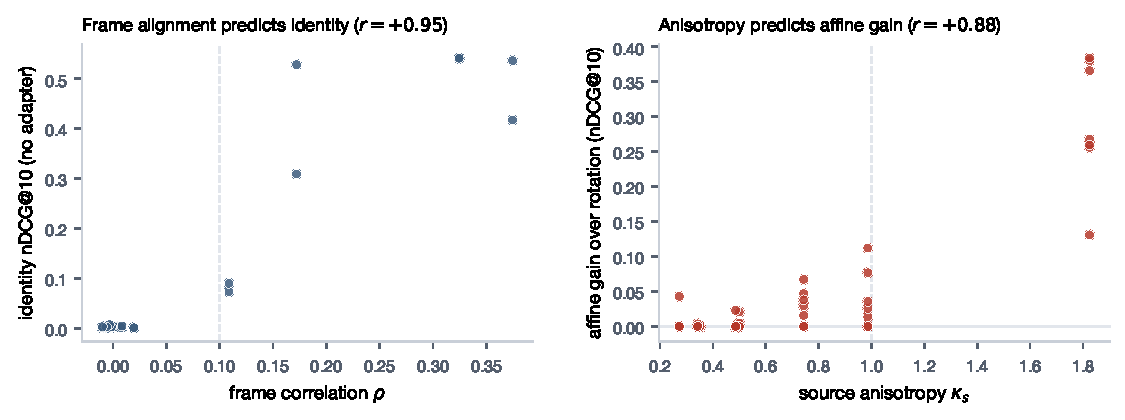
\includegraphics[width=\textwidth]{figs/diagnostics.pdf}
\caption{Pre-fit diagnostics over 56 pairs. Left: frame correlation $\rho$ predicts zero-adapter identity retrieval ($r=+0.951$). Right: source anisotropy $\kappa_s$ predicts the gain of affine alignment over pure rotation ($r=+0.882$).}
\label{fig:diag}
\end{figure}

\begin{table}[t]
\centering
\caption{Correlation of pre-fit features with identity nDCG@10, map gain over identity, affine gain over rotation, and the antisymmetric part of Procrustes retention.}
\label{tab:predictors}
\begin{tabular}{lrrrr}
\toprule
feature & $r$(identity) & $r$(map gain) & $r$(affine $-$ rot) & $r$(antisym) \\
\midrule
frame correlation $\rho$ & +0.951 & -0.862 & +0.092 & +0.000 \\
source anisotropy $\kappa_s$ & +0.097 & -0.147 & +0.882 & -0.683 \\
target anisotropy $\kappa_t$ & +0.212 & -0.224 & -0.209 & +0.683 \\
linear CKA & -0.073 & +0.319 & -0.060 & +0.000 \\
10-NN agreement & -0.057 & +0.337 & -0.111 & +0.000 \\
effective rank & +0.060 & +0.095 & -0.365 & +0.000 \\
dim ratio $d_s/d_t$ & -0.071 & +0.065 & +0.080 & -0.123 \\
fit residual gap & -0.000 & +0.003 & -0.023 & +0.032 \\
\bottomrule
\end{tabular}
\end{table}

\begin{table}[t]
\centering
\caption{Mean nDCG@10 grouped by true dimensional direction ($d_s$ vs $d_t$). Dimensional expansion does not penalize orthogonal Procrustes; the directional gap reported earlier was an artefact of source anisotropy.}
\label{tab:direction}
\begin{tabular}{lrrr}
\toprule
method & expanding & compressing & difference \\
\midrule
procrustes & 0.4749 & 0.5739 & -0.0991 \\
affine & 0.5650 & 0.5786 & -0.0137 \\
ridgecca & 0.5701 & 0.5714 & -0.0013 \\
sgd-linear & 0.5346 & 0.5374 & -0.0028 \\
sgd-mlp & 0.5229 & 0.5234 & -0.0005 \\
krr-rbf & 0.5040 & 0.4489 & 0.0551 \\
\bottomrule
\end{tabular}
\end{table}

Figure~\ref{fig:diag} and Table~\ref{tab:predictors} separate the roles of frame alignment, anisotropy, and geometry. Across 56 pairs, 48 have $\rho<0.02$ and retrieve at chance under the identity map (mean 0.003); 4 pairs have $\rho\in[0.02,0.25)$ with identity score 0.250; 4 pairs have $\rho\ge 0.25$ with identity score 0.509. Shared coordinate frames occur strictly between models sharing a pretrained backbone: the XLM-R large models (v3, bge-m3, e5-large) exhibit $\rho\in[0.172,0.375]$, and the two Qwen3-0.6B models (v5-small and Qwen3-Embedding-0.6B) exhibit $\rho=0.109$. Frame correlation $\rho$ correlates $+0.951$ with identity retrieval and $-0.862$ with map gain over identity, whereas rotation-invariant CKA correlates $-0.073$ with identity retrieval. Within the 12 Jina pairs where $\rho\approx 0$, CKA correlates $+0.743$ with affine retention, explaining why CKA appeared predictive in single-vendor evaluations.

Grouping pairs by true embedding dimension $d_s$ versus $d_t$ (Table~\ref{tab:direction}) shows that dimensional expansion does not degrade orthogonal Procrustes: expanding pairs ($d_s<d_t$, 17 pairs) average 0.5240 versus 0.4734 for compressing pairs ($d_s>d_t$, 17 pairs), and under validation-selected affine alignment expanding (0.5400) and compressing (0.5346) are within 0.0054. Instead, directional asymmetry is governed by anisotropy: under uncentred Procrustes, 44.1\% of retention variance is antisymmetric and correlates $-0.683$ with $\kappa_s$ and $+0.683$ with $\kappa_t$. Under validation-selected affine alignment, antisymmetric variance drops by 88\% to just 5.3\%.

\subsection{Deployment: query-side, corpus-side, role calibration, and hybrid migration}
\label{sec:deployment}

\begin{figure}[t]
\centering
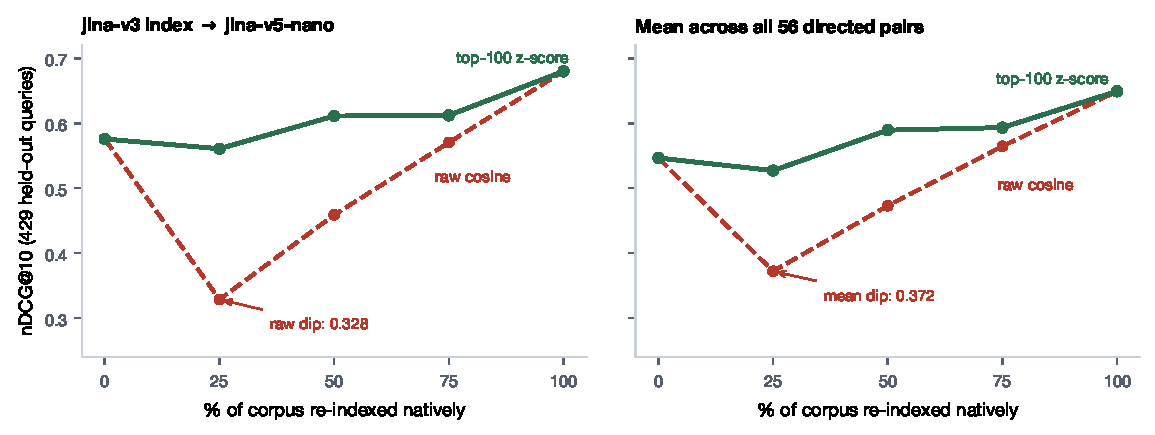
\includegraphics[width=\textwidth]{figs/progressive_migration.pdf}
\caption{Progressive zero-downtime migration from a legacy index to native target vectors (0\% to 100\% re-indexed). Left: migrating a jina-v3 index to jina-v5-nano. Right: mean across all 56 pairs. Raw cosine scoring in a mixed index collapses at 25\% migration because adapted vectors exhibit a lower background cosine mean and attenuated peak; top-100 per-shard z-scoring restores a monotone curve.}
\label{fig:hybrid}
\end{figure}

\begin{table}[t]
\centering
\caption{Progressive hybrid migration (nDCG@10 versus fraction of corpus re-indexed natively), comparing raw cosine mixing against per-query top-100 z-score merging.}
\label{tab:hybrid}
\begin{tabular}{lrrrrr}
\toprule
scenario & 0\% & 25\% & 50\% & 75\% & 100\% \\
\midrule
v3 index $\to$ v5-nano (raw cosine) & 0.5757 & 0.3284 & 0.4587 & 0.5703 & 0.6800 \\
v3 index $\to$ v5-nano (top-100 z-score) & 0.5757 & 0.5607 & 0.6111 & 0.6121 & 0.6800 \\
v5-nano index $\to$ v3 (raw cosine) & 0.5530 & 0.3694 & 0.4687 & 0.5659 & 0.6401 \\
v5-nano index $\to$ v3 (top-100 z-score) & 0.5530 & 0.5226 & 0.5952 & 0.6025 & 0.6401 \\
\midrule
Mean over 56 pairs (raw cosine) & 0.5464 & 0.3718 & 0.4729 & 0.5645 & 0.6492 \\
Mean over 56 pairs (top-100 z-score) & 0.5464 & 0.5270 & 0.5893 & 0.5933 & 0.6492 \\
\bottomrule
\end{tabular}
\end{table}

\begin{table}[t]
\centering
\caption{Role-matched calibration ablation averaged over 56 pairs. Mixing both query and passage roles outperforms single-role calibration even at matched sample count ($n=2{,}500$).}
\label{tab:role}
\begin{tabular}{lrrrr}
\toprule
calibration set & query (rot) & query (aff) & corpus (rot) & corpus (aff) \\
\midrule
Mixed (2,500 query + 2,500 passage) & 0.4998 & 0.5162 & 0.5009 & 0.5464 \\
Mixed (1,250 query + 1,250 passage) & 0.4842 & 0.4979 & 0.4854 & 0.5326 \\
Query-role only (2,500) & 0.4782 & 0.4959 & 0.4797 & 0.5337 \\
Passage-role only (2,500) & 0.4753 & 0.4609 & 0.4767 & 0.5223 \\
\bottomrule
\end{tabular}
\end{table}

Consider a production corpus frozen in jina-v3 (1024d) that an operator wants to search with jina-v5-nano (768d) queries without neural re-encoding. Two deployments solve this: adapting incoming v5-nano queries into the untouched v3 index (\texttt{v5nano->v3}), which reaches 0.5724 under Procrustes and 0.5708 under affine against 0.6401 native v3; or transforming the stored v3 vectors once by matrix multiplication into v5-nano space (\texttt{v3->v5nano} corpus-side), which reaches 0.5762 under Procrustes and 0.5757 under affine. In the reverse direction, legacy v3 queries searching a new v5-nano index reach 0.5509 query-side and 0.5530 corpus-side. Across all 56 pairs, query-side and corpus-side orthogonal Procrustes are nearly identical (0.4998 vs 0.5009), as expected from orthogonality; for fixed \texttt{affine-cs}, however, corpus-side conversion (0.5464) beats query-side (0.5162) by $+0.0302$, because shifting every document by $+\boldsymbol{\mu}_Y$ places adapted documents inside the target passage cone rather than biasing queries.

Table~\ref{tab:role} tests calibration roles. Mixing 2{,}500 query-mode and 2{,}500 passage-mode texts gives the highest accuracy on both query-side and corpus-side deployments. At matched size ($n=2{,}500$), mixed calibration still outperforms single-role calibration on query-side affine (0.4979 vs 0.4959 query-only and 0.4609 passage-only), showing that covering both query and passage subspaces prevents prompt-induced distribution shift.

A critical operational hazard arises during progressive re-indexing, when an operator re-embeds a fraction of documents natively into the new model while keeping the remaining documents corpus-adapted in one mixed index. As shown in Figure~\ref{fig:hybrid} and Table~\ref{tab:hybrid}, raw cosine search across a mixed index crashes sharply at 25\% re-indexing: v3 to v5-nano falls from 0.5757 at 0\% to 0.3284 at 25\% ($-0.2473$), and the 56-pair mean falls from 0.5464 to 0.3718 ($-0.1746$). On validation queries for v3 to v5-nano, native v5-nano documents have a background cosine mean of 0.2035 and a relevant-document mean of 0.4153, whereas adapted v3 documents have a background mean of 0.0827 and a relevant mean of 0.2458; irrelevant native documents therefore outscore relevant adapted documents. Querying the native and adapted shards separately and normalizing each shard's top-100 cosine scores to zero mean and unit variance per query eliminates the crash without extra model calls: v3 to v5-nano rises from 0.3284 to 0.5607 at 25\% and 0.6111 at 50\%, and the 56-pair mean recovers from 0.3718 to 0.5270 at 25\% and 0.5893 at 50\%.

\subsection{Chaining, a shared Platonic hub, low-rank compression, and dark memories}
\label{sec:structure}

\begin{figure}[t]
\centering
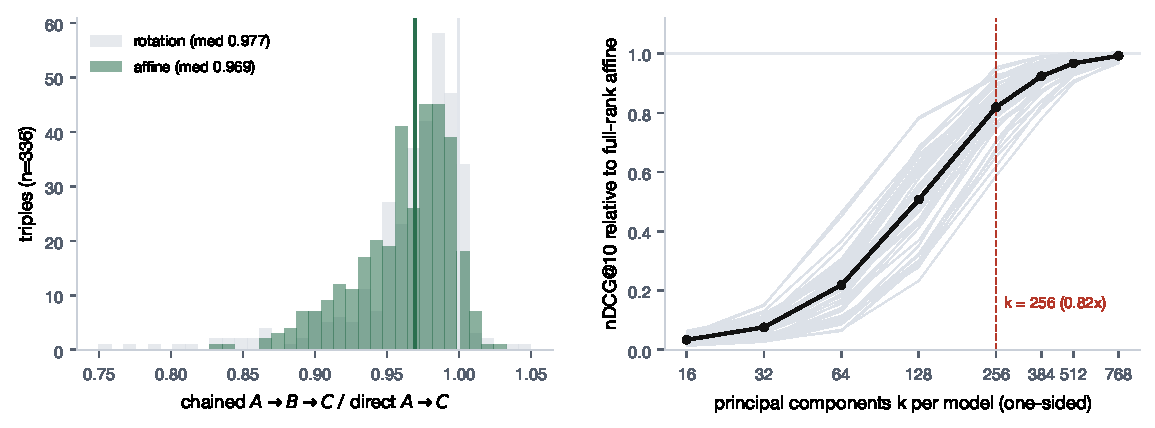
\includegraphics[width=\textwidth]{figs/structure.pdf}
\caption{Left: two-hop chained maps $A\to B\to C$ relative to direct $A\to C$ over all 336 ordered triples. Right: one-sided low-rank affine compression (zero corpus re-indexing) across $k\in[16,768]$ principal components per model; thin lines show all 56 pairs and the bold line shows their mean.}
\label{fig:structure}
\end{figure}

\begin{table}[t]
\centering
\footnotesize
\setlength{\tabcolsep}{4pt}
\begin{minipage}[t]{0.42\linewidth}
\centering
\caption{One-sided low-rank affine compression over 56 pairs (no corpus modification).}
\label{tab:lowrank}
\begin{tabular}{rrrr}
\toprule
rank $k$ & nDCG@10 & relative to full & pairs \\
\midrule
16 & 0.0176 & 0.034 & 56 \\
32 & 0.0403 & 0.076 & 56 \\
64 & 0.1171 & 0.219 & 56 \\
128 & 0.2688 & 0.507 & 56 \\
256 & 0.4265 & 0.819 & 56 \\
384 & 0.4782 & 0.924 & 56 \\
512 & 0.4998 & 0.967 & 56 \\
768 & 0.5127 & 0.993 & 56 \\
\bottomrule
\end{tabular}
\end{minipage}\hfill
\begin{minipage}[t]{0.55\linewidth}
\centering
\caption{Calibration budget $n$ over 56 pairs.}
\label{tab:calsize}
\begin{tabular}{rrrrr}
\toprule
$n$ & Procrustes & Affine (fixed) & Source-centred & Ridge \\
\midrule
50 & 0.0287 & 0.0202 & 0.0314 & 0.0285 \\
100 & 0.0904 & 0.0716 & 0.1104 & 0.0938 \\
250 & 0.2650 & 0.2418 & 0.3064 & 0.2525 \\
500 & 0.3780 & 0.3727 & 0.4263 & 0.3587 \\
1,000 & 0.4440 & 0.4523 & 0.4877 & 0.4367 \\
2,500 & 0.4842 & 0.4979 & 0.5215 & 0.4816 \\
5,000 & 0.4998 & 0.5162 & 0.5336 & 0.4980 \\
\bottomrule
\end{tabular}
\end{minipage}
\end{table}

\paragraph{Chaining.} Over all 336 ordered triples $(A,B,C)$, composing $A\to B$ and $B\to C$ without running model $B$ retains a median 0.977 of direct $A\to C$ under orthogonal Procrustes (80.7\% of triples above 0.95, p10 0.918) and 0.970 under fixed affine (70.2\% above 0.95, p10 0.914, Figure~\ref{fig:structure}, left).

\paragraph{One shared Platonic hub.} Fitting a single Generalized Procrustes Analysis (GPA) hub in $\mathbb{R}^{2048}$ across all eight models using all 5{,}000 calibration texts and 40 iterations requires only 8 maps instead of 56 pairwise maps. Contrary to earlier under-converged subsets, a converged hub matches pairwise fitting across every variant: uncentred GPA averages 0.4996 against 0.4998 pairwise ($\Delta=-0.0002$, winning 23/56 pairs), Affine GPA averages 0.5165 against 0.5162 pairwise ($\Delta=+0.0002$, winning 26/56), and source-centred GPA averages 0.5345 against 0.5336 pairwise ($\Delta=+0.0009$, winning 34/56 pairs). Eight independently trained models across six vendors and three embedding widths thus embed cleanly into a single shared orthogonal coordinate frame with zero retrieval penalty.

\paragraph{One-sided low-rank compression.} Projecting both centred calibration matrices onto their top $k$ principal components, solving a $k\times k$ orthogonal Procrustes problem, and lifting back into target space leaves the corpus untouched (Table~\ref{tab:lowrank} and Figure~\ref{fig:structure}, right). Mean retention relative to full-rank affine rises monotonically from 0.034 at $k=16$ to 0.507 at $k=128$, 0.819 at $k=256$, 0.924 at $k=384$, 0.967 at $k=512$, and 0.993 at $k=768$, closely paralleling the 256-component knee reported for LLM hidden states \citep{platoskey2026}.

\paragraph{Recoverable failures and compute cost.} Over aligned top-10 hit sets, source-centred Procrustes recovers a mean 0.258 (range 0.138 to 0.488) of relevant documents that only the source model retrieves while losing 0.282 of native target hits; validation-selected affine recovers 0.255 while losing 0.272, and uncentred Procrustes recovers 0.235 while losing 0.338. On CPU for v5-nano to v3 ($768\to 1024$, $n=5{,}000$), fitting takes 302\,ms for Procrustes and 338\,ms for affine, single-query mapping takes 75.8\,$\mu$s, and transforming 100{,}000 corpus vectors takes 1.05\,s (10.5\,s per million vectors), orders of magnitude cheaper than neural re-encoding.

\section{Discussion and limitations}

An embedding adapter is a bridge, not a free upgrade. Across 56 directed pairs from six vendors, even the strongest one-sided closed-form map recovers 0.841 of the source index's nDCG@10 on average and outperforms the old index only between consecutive checkpoints of the same lineage. Its practical value is operational continuity: serving queries from a newly deployed model against a frozen legacy index at 76\,$\mu$s per query, keeping legacy clients working against a newly indexed corpus, or running zero-downtime progressive re-indexing once per-shard top-100 z-score normalization prevents the mixed-index cosine crash.

Three engineering rules follow directly from our measurements. First, compute $\rho$ and $\kappa$ on 1{,}000 to 5{,}000 mixed query-and-passage calibration pairs before choosing a map. Second, when no labeled validation queries exist, default to source-centred Procrustes (Equation~\eqref{eq:src_centred}) for query-side serving and affine alignment for corpus-side conversion; when a small validation set exists, select centring and scale on validation nDCG@10. Third, when serving a multi-model fleet, fit one converged source-centred GPA hub (8 maps instead of $M(M-1)$) at zero retrieval cost.

NanoBEIR contains 50 queries per task (429 held-out queries per split), so per-pair differences below 0.02 nDCG@10 remain noisy even though five-seed aggregate standard deviations are 0.008. Calibration uses English AG News exclusively; domain-matched or multilingual calibration may further narrow the gap to native retrieval. Finally, all eight models are dense single-vector encoders; multi-vector late-interaction models such as ColBERT remain outside this study.

\section{Related work}

Orthogonal Procrustes alignment on paired vectors originated in cross-lingual word embedding alignment \citep{conneau2018word,artetxe2018vecmap}, with unpaired Wasserstein-Procrustes \citep{grave2018wasserstein} and multilingual hyperalignment \citep{alaux2019umh} extending it to unaligned and multi-space settings. For dense text retrieval, \citet{vejendla2025drift} compare closed-form rotations against low-rank affine maps and residual MLPs on a million-item index, \citet{zhao2026bill} benchmark 14 pairs against the source index to establish migration break-even points, \citet{maekawa2026align} evaluate closed-form baselines alongside symmetric adaptation on MAIR, \citet{yoon2025converter} train four-layer converters across BEIR, and \citet{chivukula2026era} train anchor-based replacement adapters. Multi-way representation alignment \citep{achara2026multiway} contrasts generalized Procrustes hubs against non-isometric multiset CCA on translation tasks, while relative representations \citep{moschella2023relative}, adversarial cycle-consistent translation \citep{jha2025vec2vec}, and spectral contrastive alignment \citep{sui2026unicon} address unpaired or kernelized regimes. Finally, Plato's Key \citep{platoskey2026} and latent space stitching \citep{maiorca2023latent} demonstrate that simple orthogonal and affine coordinate changes transfer functional behaviour across independently trained neural networks without gradient descent.

\bibliographystyle{plainnat}
\begin{thebibliography}{99}

\bibitem[Achara et al.(2026)]{achara2026multiway}
Achara, A. et al. (2026). Multi-way representation alignment. arXiv:2602.06205.

\bibitem[Alaux et al.(2019)]{alaux2019umh}
Alaux, J., Grave, E., Cuturi, M., Joulin, A. (2019). Unsupervised hyperalignment for multilingual word embeddings. ICLR.

\bibitem[Artetxe et al.(2018)]{artetxe2018vecmap}
Artetxe, M., Labaka, G., Agirre, E. (2018). A robust self-learning method for fully unsupervised cross-lingual mappings of word embeddings. ACL. arXiv:1805.06297.

\bibitem[Cheng et al.(2026)]{platoskey2026}
Cheng, V., Liu, J., Yau, M., R\'e, C. (2026). Plato's Key. HazyResearch, 25 November 2026.

\bibitem[Chivukula et al.(2026)]{chivukula2026era}
Chivukula, et al. (2026). ERA: embedding replacement adapters. arXiv:2611.26919.

\bibitem[Conneau et al.(2018)]{conneau2018word}
Conneau, A., Lample, G., Ranzato, M., Denoyer, L., J\'egou, H. (2018). Word translation without parallel data. ICLR. arXiv:1710.04087.

\bibitem[Grave et al.(2019)]{grave2018wasserstein}
Grave, E., Joulin, A., Berthet, Q. (2019). Unsupervised alignment of embeddings with Wasserstein Procrustes. AISTATS. arXiv:1805.11222.

\bibitem[Jha et al.(2025)]{jha2025vec2vec}
Jha, et al. (2025). vec2vec: text embeddings are secretly aligned. NeurIPS. arXiv:2505.12540.

\bibitem[Maekawa et al.(2026)]{maekawa2026align}
Maekawa, et al. (2026). Align then adapt. EMNLP. arXiv:2604.03403.

\bibitem[Maiorca et al.(2023)]{maiorca2023latent}
Maiorca, V., Moschella, L., Norelli, A., Fumero, M., Locatello, F., Rodol\`a, E. (2023). Latent space translation via semantic alignment. NeurIPS. arXiv:2311.00664.

\bibitem[Moschella et al.(2023)]{moschella2023relative}
Moschella, L., Maiorca, V., Fumero, M., Norelli, A., Locatello, F., Rodol\`a, E. (2023). Relative representations enable zero-shot latent space communication. ICLR. arXiv:2209.15430.

\bibitem[Sui et al.(2026)]{sui2026unicon}
Sui, H., Wang, Y., Do, M. N. (2026). UniCon: unified framework for efficient contrastive alignment via kernels. ICLR. arXiv:2604.16678.

\bibitem[Vejendla(2025)]{vejendla2025drift}
Vejendla, (2025). Drift-Adapter. EMNLP. arXiv:2509.23471.

\bibitem[Xiao(2026)]{xiao2026adapters}
Xiao, H. (2026). Cross-model embedding adapters: forward and backward compatibility without re-embedding. Technical report.

\bibitem[Yoon and Ar{\i}k(2025)]{yoon2025converter}
Yoon, J., Ar{\i}k, S. \"O. (2025). Embedding converter. ACL.

\bibitem[Zhao et al.(2026)]{zhao2026bill}
Zhao, et al. (2026). When the bill falls due. arXiv:2611.20702.

\end{thebibliography}

\clearpage
\appendix
\section{Full 8$\times$8 retrieval matrices}

\begin{table}[ht]
\centering
\caption{Adapted nDCG@10 on the 429 held-out queries under validation-selected affine alignment (Plato's Key). Diagonal entries show native model scores.}
\label{tab:matrix_affine}
\begin{tabular}{lrrrrrrrr}
\toprule
source $\backslash$ target & v5s & v5n & q3 & arc & v4 & v3 & bge & e5 \\
\midrule
v5s & \textit{0.682} & 0.674 & 0.619 & 0.500 & 0.619 & 0.576 & 0.550 & 0.568 \\
v5n & 0.681 & \textit{0.680} & 0.619 & 0.509 & 0.624 & 0.571 & 0.554 & 0.568 \\
q3 & 0.636 & 0.630 & \textit{0.656} & 0.455 & 0.611 & 0.574 & 0.544 & 0.544 \\
arc & 0.487 & 0.496 & 0.455 & \textit{0.653} & 0.494 & 0.470 & 0.434 & 0.464 \\
v4 & 0.624 & 0.614 & 0.575 & 0.476 & \textit{0.653} & 0.532 & 0.502 & 0.542 \\
v3 & 0.562 & 0.551 & 0.532 & 0.471 & 0.549 & \textit{0.640} & 0.593 & 0.577 \\
bge & 0.524 & 0.521 & 0.469 & 0.408 & 0.477 & 0.594 & \textit{0.616} & 0.592 \\
e5 & 0.565 & 0.560 & 0.533 & 0.453 & 0.502 & 0.588 & 0.572 & \textit{0.615} \\
\bottomrule
\end{tabular}
\end{table}

\begin{table}[ht]
\centering
\caption{Adapted nDCG@10 on the 429 held-out queries under orthogonal Procrustes. Diagonal entries show native model scores.}
\label{tab:matrix_proc}
\begin{tabular}{lrrrrrrr}
\toprule
source $\backslash$ target & v5s & v5n & q3-0.6 & v4 & v3 & e5l & bm3 \\
\midrule
v5s & \textit{0.682} & 0.674 & 0.618 & 0.619 & 0.572 & 0.568 & 0.550 \\
v5n & 0.684 & \textit{0.680} & 0.619 & 0.624 & 0.572 & 0.569 & 0.554 \\
q3-0.6 & 0.631 & 0.628 & \textit{0.654} & 0.612 & 0.552 & 0.543 & 0.543 \\
v4 & 0.598 & 0.600 & 0.540 & \textit{0.653} & 0.456 & 0.542 & 0.503 \\
v3 & 0.562 & 0.551 & 0.532 & 0.549 & \textit{0.640} & 0.577 & 0.593 \\
e5l & 0.306 & 0.292 & 0.149 & 0.246 & 0.207 & \textit{0.615} & 0.443 \\
bm3 & 0.486 & 0.491 & 0.454 & 0.477 & 0.546 & 0.592 & \textit{0.616} \\
\bottomrule
\end{tabular}
\end{table}

\end{document}
